El proyecto de investigación marco tiene como objetivo desarrollar Microrredes (MG) y tecnologías de almacenamiento (ESS) que permitan el uso eficiente de la energía eléctrica  para aumentar la cobertura y confiabilidad del servicio en zonas no interconectadas \cite{microgrid}.

El propósito de las MG es integrar fuentes de energía convencionales y no convencionales para contribuir en la mejora de la calidad de servicio en donde la continuidad se ve afectada por las fallas de la red de distribución. Por otra parte, la mitigación de gases de efecto invernadero es de suma importancia para el desarrollo sostenible medioambiental en donde la incorporación de tecnologías energéticas sostenibles son relevantes en el desarrollo de las microrredes. Por lo tanto, se realizará una implementación  piloto de MG basado en sistemas de generación diésel y ESS integrado a una plataforma de red inteligente para el control, monitoreo y supervisión del sistema con el objetivo de identificar la relación óptima de capacidad entre la generación con recursos energéticos distribuidos, plantas Diésel y ESS   \cite{microgrid}.

La implementación de la microrred busca prestar servicios complementarios para incrementar la cobertura, eficiencia energética y confiabilidad del servicio en el departamento de Cundinamarca \cite{microgrid}. Para ello, el proyecto marco se desarrollará en las siguientes fases (Figura 1):
\newpage
\begin{figure}[h!]
    \begin{center}
    \centering
    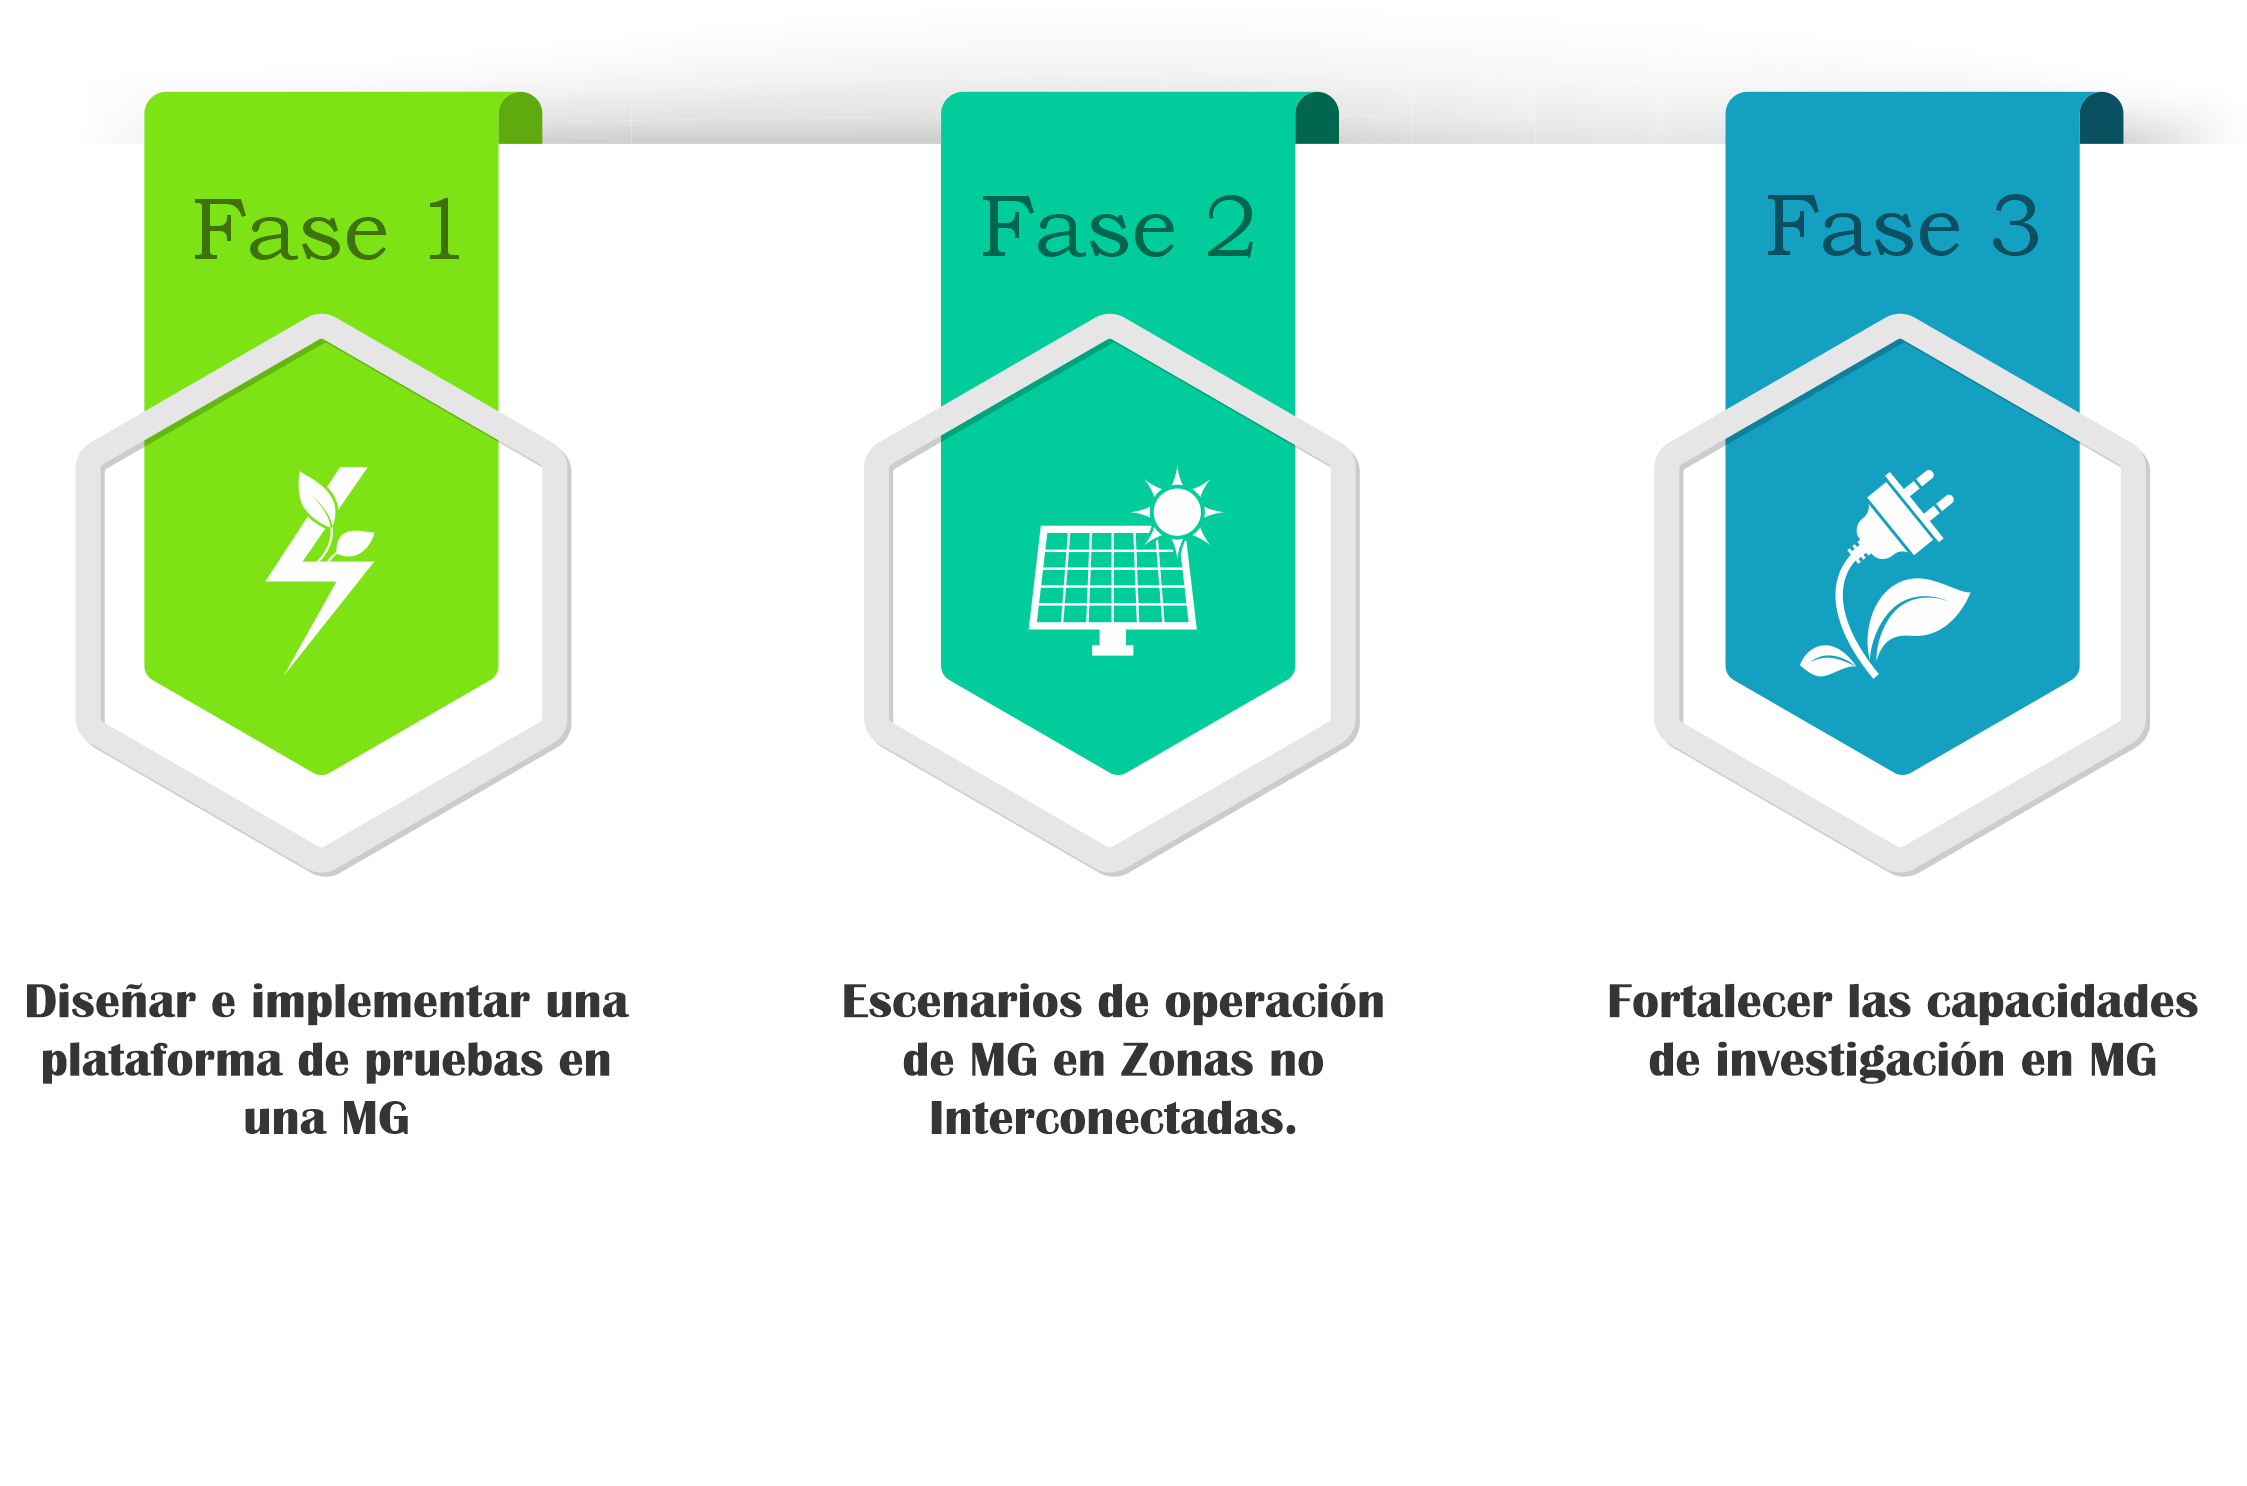
\includegraphics[scale=0.75]{Imágenes/contexto/Fases.png}
	\caption{ Fases proyecto marco}
    \end{center}
\end{figure}

\textbf{Fase 1: } Consulta de revistas especializadas, normas y artículos con el objeto de realizar pruebas enfocadas en las variables más relevantes que monitorean la MG para realizar una adquisición de datos que logre determinar los puntos óptimos de operación de la microrred.\\

\textbf{Fase 2: } Desarrollo de  modelos en simulación que permita establecer el comportamiento de la MG en diferentes escenarios, con el fin de desarrollar  artículos de investigación que permitan la presentación de los resultados obtenidos del proyecto.\\

\textbf{Fase 3: } Realizar capacitaciones acerca de las MG para garantizar su funcionamiento,  elaborando manuales de operación referente a la investigación, con la finalidad de ejecutar el proyecto de manera eficiente.


El trabajo de grado aportará al proyecto marco en la fase 2 mediante la investigación acerca del comportamiento en tecnologías de baterías existentes en el mercado considerando la  interacción con la red eléctrica bajo fenómenos de calidad de potencia. La investigación se realizará a través de revisión bibliográfica en fuentes verídicas tales como revistas indexadas, trabajos de grado, artículos científicos e información de instituciones vinculadas al proyecto para posteriormente establecer escenarios de pruebas mediante simulación.